\documentclass[main.tex]{subfiles}

\begin{document}

\chapter{The combined \gls{sd} spectrum}
\label{chapter:sd750_combined_spectrum}

This chapter presents an updated measurement of the \sd{750} spectrum and its combination with the \sd{433} spectrum.
The \sd{750} analysis builds on the spectrum published in 2021~\cite{PierreAuger:2021:InfillSpectrum} and uses an updated dataset.
The detection efficiency is revisited with a data-driven method based on the fraction of \sd{433} events also detected by the \sd{750}, as described in \cref{subsec:sd750_efficiency}.
Together with the energy bias and resolution from Ref.~\cite{PierreAuger:2021:InfillSpectrum}, this efficiency defines the detector response used to unfold the updated \sd{750} spectrum in \cref{subsec:sd750_spectrum}.
Finally, in \cref{sec:combined_spectrum}, the separately reconstructed \sd{433} and \sd{750} measurements are combined using a likelihood method.
The stability of the combined result is assessed, and all spectral parameters from the second knee through the ankle are determined.

\section{The \sd{750} Spectrum}
\label{sec:sd750_spectrum}

\subsection{The \sd{750} dataset}

In 2021, the Pierre Auger Collaboration measured the cosmic-ray spectrum with approximately $\num{560000}$ \sd{750} events above $10^{17}\,\mathrm{eV}$~\cite{PierreAuger:2021:InfillSpectrum}.
The measurement revealed a turn-down close to its lower energy boundary and extended up to $\lg(E/\mathrm{eV})=19.5$, thereby including the ankle.
Because the break energy was close to the analysis threshold and the transition extended over a broad energy range, the low-energy side of the feature could not be fully characterized.
In particular, the second-knee energy and the spectral index below the break were only inferred indirectly.

The \sd{750} Phase I dataset used in this analysis spans January 2014, following the introduction of the Gen.~II triggers \gls{totd} and \gls{mops}, to 29 November 2021, when the transition to the upgraded electronics began.
This adds more than three years of data relative to the dataset used for the spectrum published in 2021.
The shower geometry is reconstructed as described in \cref{subsec:geometry_ldf}, using Herald because the Observer reconstruction was not updated for the \sd{750}.
Events are required to satisfy the fiducial 6T5 trigger, ensuring adequate containment of the shower footprint around the station with the largest signal.
As in the published analysis, the spectrum measurement is restricted to $\theta<40^\circ$, for which the Gen.~II triggers provide strong sensitivity to the electromagnetic shower component.
Periods affected by acquisition problems are excluded.
As for the \sd{433}, the exposure is calculated from the number of active hexagons, yielding $\mathcal{E}_{\text{SD-750}}=$\SDSevenFiftyExposure above the full-efficiency threshold.

\subsection{\sd{750} efficiency and response function}
\label{subsec:sd750_efficiency}

The \sd{750} efficiency was previously estimated using a limited sample of hybrid events observed by Coihueco and through simulations~\cite{2018:Coleman:Thesis}.
Because the \sd{433} is nested within the \sd{750}, the efficiency can instead be estimated from the fraction of \sd{433} events also detected by the \sd{750}.
Although the reconstructed energy scales of the two arrays are related, this does not prevent the determination of the full-efficiency threshold, which is the main objective of this study.
The same data are used to parameterize the efficiency below the threshold, where its effect enters through the forward-folding procedure and has only a minor influence on the resulting spectrum.
Using periods during which both arrays were active in Phase I, the binned \sd{750} efficiency is estimated as
\begin{align}
    \varepsilon(E_i)=\frac{k_i}{n_i},
\end{align}
\noindent where $n_i$ is the number of events detected by the \sd{433} in energy bin $i$, and $k_i$ is the subset of those events also detected by the \sd{750}.
Events are matched using their unique identifiers and cross-checked using their GPS times, following the procedure adopted for the calibration.
The filled circles in \cref{fig:sd750_efficiency} show the resulting efficiencies, with error bars representing the $68\%$ Clopper--Pearson confidence intervals~\cite{Clopper:1934:BinomialInterval}.
Only energies above the full-efficiency threshold of the \sd{433} are included.

\begin{figure}
    \centering
    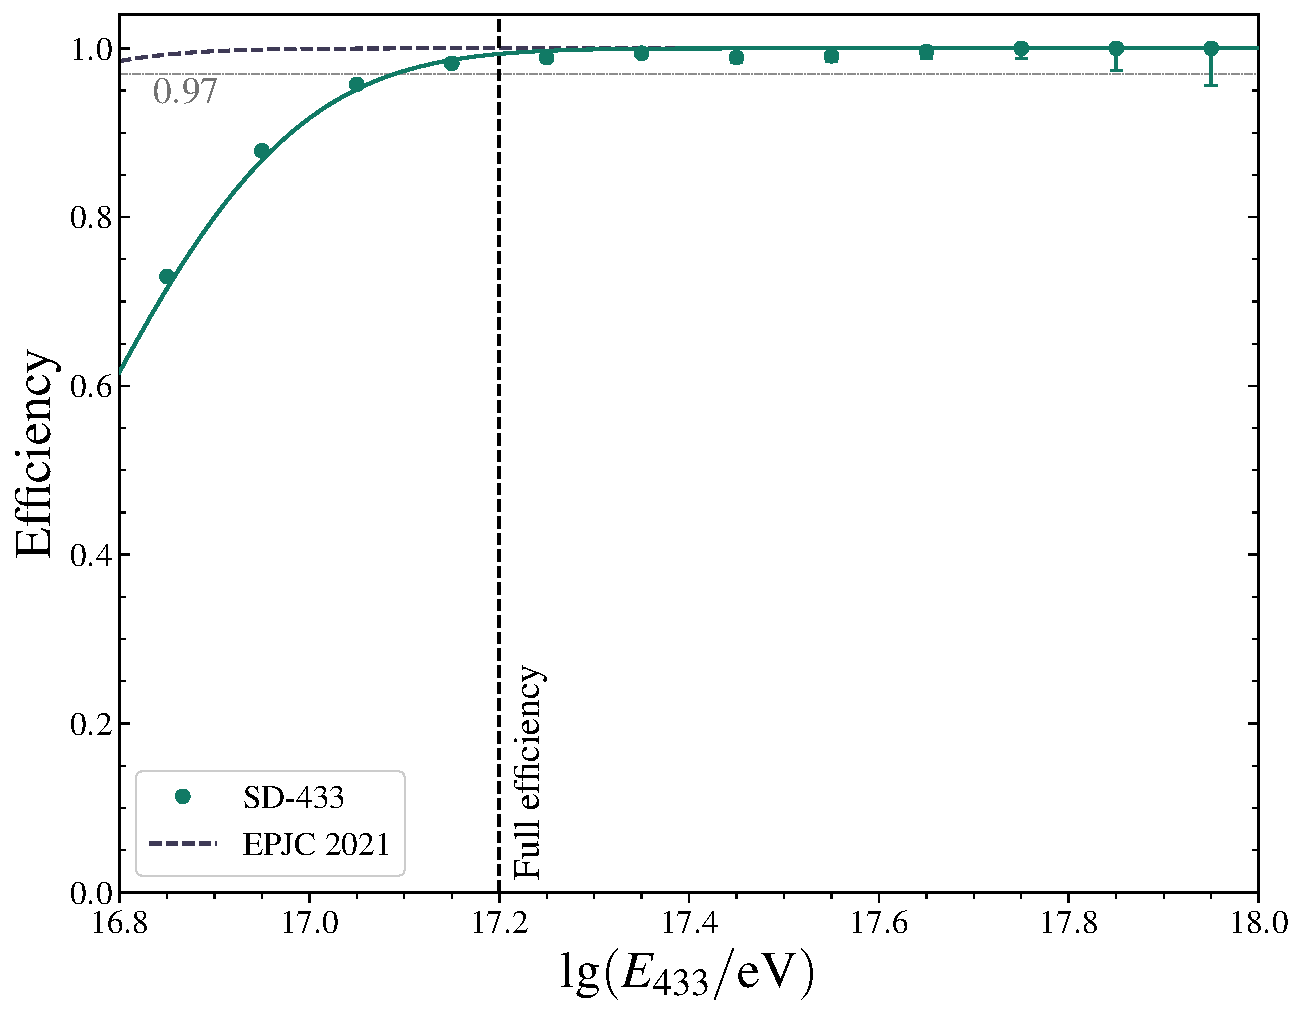
\includegraphics[width=0.8\linewidth]{figures/chapter_combined/sd750_efficiency.pdf}
    \caption{Reconstruction efficiency of the \sd{750} as a function of the energy reconstructed with the \sd{433}. The filled markers show the efficiency obtained with the updated dataset, while the open markers show the efficiency reported in the previous \sd{750} spectrum measurement~\cite{PierreAuger:2021:InfillSpectrum}. The horizontal dashed line indicates an efficiency of $0.97$.}
    \label{fig:sd750_efficiency}
\end{figure}
The Clopper--Pearson construction gives a one-sided lower limit when all events in a bin are detected, $k_i=n_i$, thereby respecting the physical bound $\varepsilon\leq1$.
To parameterize the efficiency, a binomial likelihood fit was used, where for each bin,
\begin{align}
    \mathcal{L}(\mu,\sigma)
    =
    \prod_{i=1}^{N_{\mathrm{bins}}}
    \binom{n_i}{k_i}
    \varepsilon_i^{k_i}
    (1-\varepsilon_i)^{n_i-k_i},
\end{align}
\noindent where $\varepsilon_i=\varepsilon(E_i;\mu,\sigma)$.
Following Ref.~\cite{PierreAuger:2021:InfillSpectrum}, the efficiency is modeled as
\begin{align}
    \varepsilon(E)
    =
    \frac{1}{2}
    \left[
    1+\mathrm{erf}
    \left(
    \frac{\lg(E/\mathrm{eV})-\mu}{\sigma}
    \right)
    \right],
\end{align}
\noindent where $\mu$ determines the position of the transition and $\sigma$ its width.
The best-fit values are $\mu=16.74\pm0.01$ and $\sigma=0.250\pm0.001$, with correlation $\rho_{\mu,\sigma}=0.38$.
The fitted curve is shown as a solid line in \cref{fig:sd750_efficiency}, while the dashed line shows the result from Ref.~\cite{PierreAuger:2021:InfillSpectrum}.
Defining full efficiency at $\varepsilon=0.97$ gives a threshold of $\lg(E/\mathrm{eV})=17.2$, marked by the vertical gray line.
The updated threshold lies approximately two energy bins above the previous estimate.

The \sd{750} energy bias and resolution are required to construct its migration matrix.
We adopt the parameterizations used in Ref.~\cite{PierreAuger:2021:InfillSpectrum}.
The left panel of \cref{fig:sd433_sd750_response} compares the relative energy biases of the two arrays.
For the \sd{750}, the bias is modeled as
\begin{align}
    b(E)=b_0(x-b_1)\exp
    \left[
    -b_2(x-b_3)^2
    \right]+b_4,
    \label{eq:sd750_bias}
\end{align}
\noindent where $x=\lg(E/\mathrm{eV})$.
The best-fit parameters are
\begin{align*}
    \begin{gathered}
        b_0 = -3 \pm 1, \qquad
        b_1 = 26 \pm 4, \qquad
        b_2 = 0.35 \pm 0.02, \\[4pt]
        b_3 = 12.7 \pm 0.1, \qquad
        b_4 = -0.0039 \pm 0.0008
    \end{gathered}
\end{align*}
The \sd{433} bias is smaller in magnitude throughout the displayed energy range, while the \sd{750} bias approaches $b_4$, corresponding to approximately $-0.4\%$, at high energies.

The right panel of \cref{fig:sd433_sd750_response} compares the relative energy resolutions of the two arrays.
At lower energies, the denser spacing of the \sd{433} reduces the detector contribution and provides better energy resolution.
As the energy increases, this contribution decreases and the \sd{750} resolution approaches its shower-to-shower fluctuation term, resulting in better resolution at high energies.
The \sd{750} resolution is modeled using \cref{eq:resolution_sigma}, with $r_{\mathrm{sh}}=0.06\pm0.02$ and $r_{\mathrm{det}}=0.05\pm0.01$.

\begin{figure}
    \centering
    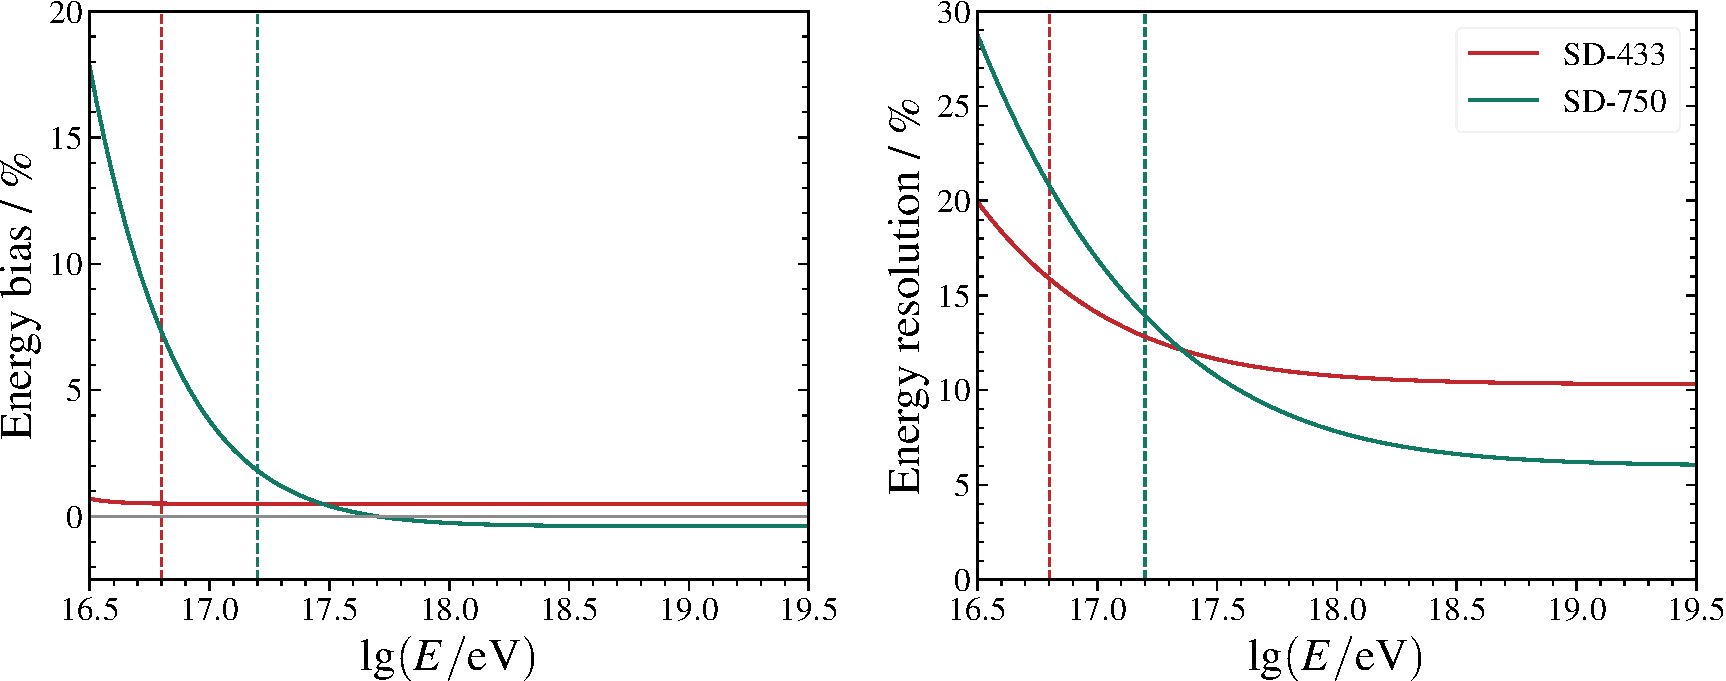
\includegraphics[width=\linewidth]{figures/chapter_combined/sd433_sd750_bias_resolution.pdf}
    \caption{Relative energy bias (left) and energy resolution (right) used to construct the \sd{433} and \sd{750} response matrices. The vertical dashed lines indicate the full-efficiency thresholds adopted for the two arrays.}
    \label{fig:sd433_sd750_response}
\end{figure}

Using the efficiency, energy bias, and resolution described above, the \sd{750} migration matrix is constructed following the formalism introduced in \cref{sec:unfolded_spectrum}.
The approximate matrix in \cref{eq:matrix_approx} is evaluated with a true-energy bin width of $\Delta\lg(E_\text{true}/\mathrm{eV})=0.01$, making it independent of the assumed spectral model.
The resulting matrix is shown in \cref{fig:sd750_migration_matrix}.
The dashed vertical line marks the \sd{750} full-efficiency threshold, and the white diagonal indicates $E_\text{true}=E_\text{rec}$.
Compared with the \sd{433} analysis, the \sd{750} migration matrix spans a wider energy range to account for migrations across the analysis boundaries.
Near the \sd{750} full-efficiency threshold, the response width is comparable to that of the \sd{433}.
At higher energies, the improved \sd{750} resolution produces a narrower response around the diagonal.
The raw event distribution can then be forward-folded through this matrix to fit the spectral model.
\begin{figure}
    \centering
    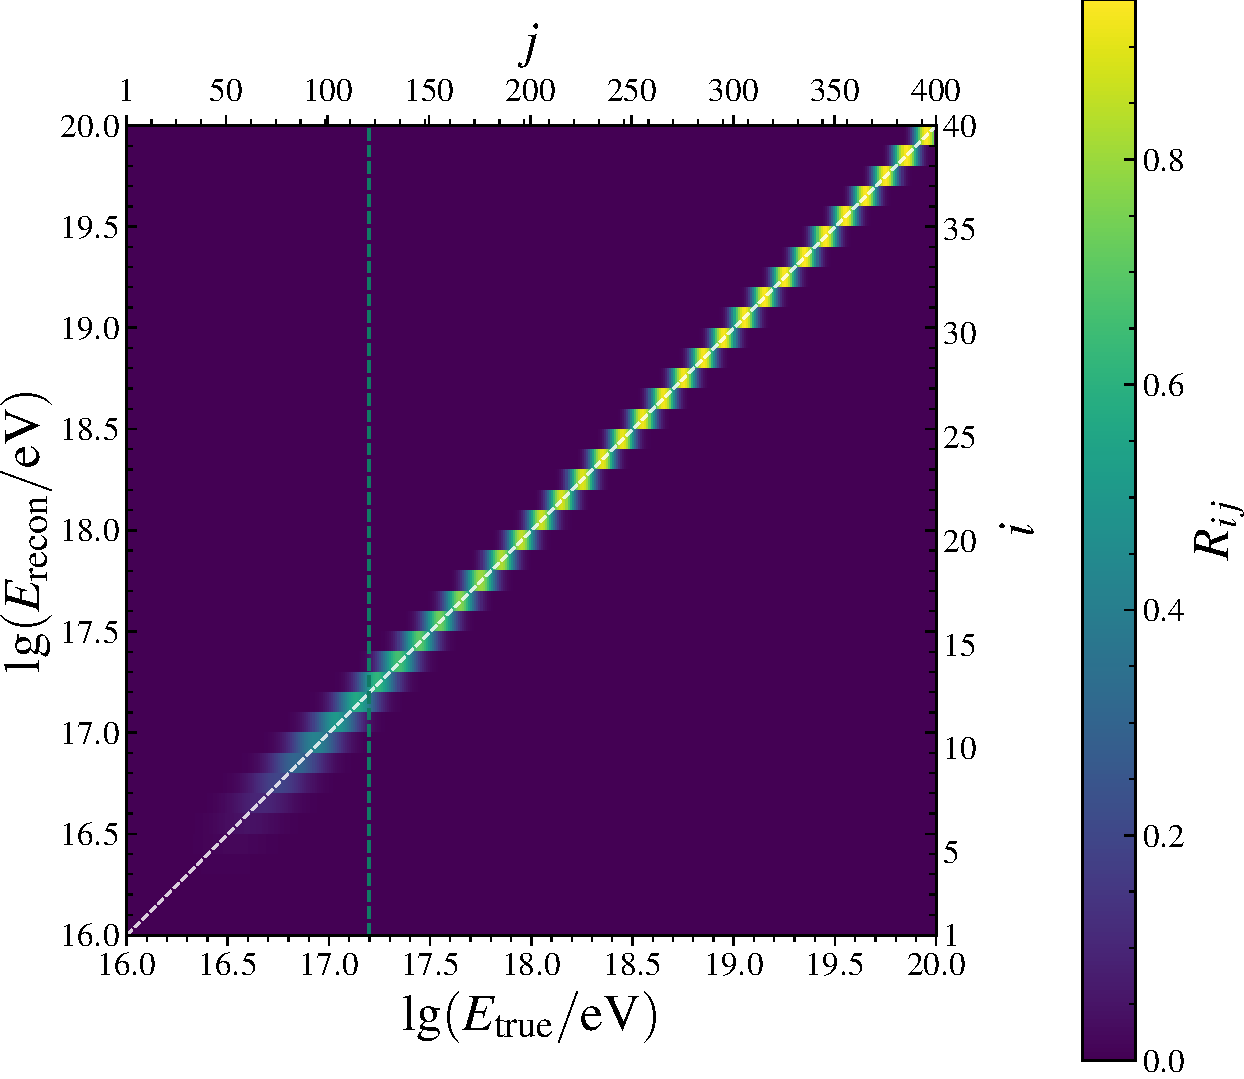
\includegraphics[width=0.78\linewidth]{figures/chapter_combined/sd750_migration_matrix.pdf}
    \caption{Migration matrix used for the updated \sd{750} spectrum. The horizontal axis gives the true-energy bin $j$ and the vertical axis the reconstructed-energy bin $i$; the additional axes give the corresponding logarithmic energies. The matrix includes the measured reconstruction efficiency, energy bias, and energy resolution.}
    \label{fig:sd750_migration_matrix}
\end{figure}

\subsection{Updated SD-750 spectrum}
\label{subsec:sd750_spectrum}

The \sd{750} events are reconstructed with Herald.
For the updated and combined spectra, their energies are recalibrated using the ICRC 2025 energy scale described in \cref{sec:calibration}.
Relative to the previous calibration, the energy changes by less than $0.5\%$ near the full-efficiency threshold and by less than $2\%$ at the highest energies.
The corresponding effect on the spectrum is therefore small.

The left panel of \cref{fig:sd750_raw_spectrum} compares the raw spectrum obtained from the updated dataset for $\theta<40^\circ$ with the spectrum published in 2021~\cite{PierreAuger:2021:InfillSpectrum}.
The updated flux differs by approximately $5\%$ over most of the energy range, primarily because periods affected by acquisition problems were inadvertently included in the earlier calculation.
This produces an approximately energy-independent normalization shift, which is more visible in the $E^3$-scaled representation in the right panel.
The smaller energy-dependent difference arises from the updated energy calibration.
When the same fit conditions are applied, the fitted spectral parameters remain compatible with the published result, as shown in \cref{appendix:chapter_combined}.
The updated dataset is also used for the \sd{433} calibration.

\begin{figure}
    \centering
    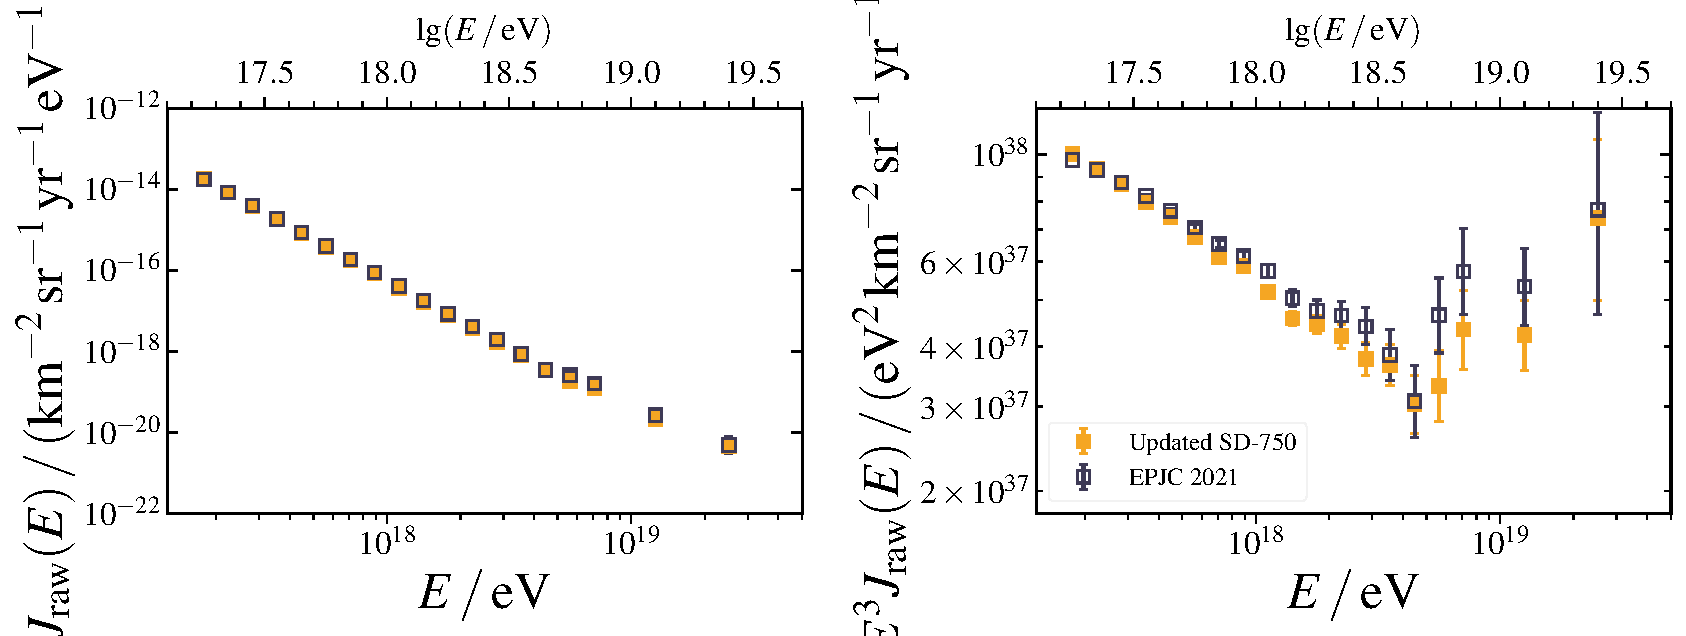
\includegraphics[width=0.9\linewidth]{figures/chapter_combined/sd750_raw_spectrum.pdf}
    \caption{Raw cosmic-ray spectrum measured with the updated \sd{750} dataset, compared with the spectrum reported in \cite{PierreAuger:2021:InfillSpectrum}. The left panel shows the differential flux and the right panel the flux multiplied by $E^3$. Both measurements are displayed using the same energy bins. Only statistical uncertainties are shown.}
    \label{fig:sd750_raw_spectrum}
\end{figure}

The spectral model is fitted by forward-folding it through the \sd{750} migration matrix shown in \cref{fig:sd750_migration_matrix}.
Owing to the larger collecting area of the \sd{750}, the measured energy range extends through the ankle, a hardening of the cosmic-ray spectrum near $4\,\mathrm{EeV}$~\cite{PierreAuger:2021:InfillSpectrum}.
The flux is therefore modeled with an extension of \cref{eq:bplwst},
\begin{align}
    J(E)=J_0
    \left(
    \frac{E}{10^{17}\,\mathrm{eV}}
    \right)^{-\gamma_0
    }
    \prod \limits_{i=0}^{1}
    \left[
    1+
        \left(
        \frac{E}{E_{ij}}
        \right)
        ^{\frac{1}{\omega_{ij}}}
    \right]^{(\gamma_i-\gamma_j)\omega_{ij}},
    \label{eq:extended_bplwst}
\end{align}
\noindent where $j=i+1$.
The parameters $E_{01}$ and $E_{12}$ give the positions of the second knee and ankle, while $\omega_{01}$ and $\omega_{12}$ determine their transition widths.
The indices $\gamma_0$, $\gamma_1$, and $\gamma_2$ describe the three intervening power-law regimes.
Because the ankle transition is sharp, $\omega_{12}$ is fixed to $0.05$ in the fit.

Because the \sd{750} full-efficiency threshold lies close to the second knee, the standalone data cannot constrain all spectral parameters simultaneously.
The second-knee position is therefore fixed to the \sd{433} result in the fit, while its transition width remains free.
As a cross-check, allowing the position to vary gives $\lg(E_{01}/\mathrm{eV})=17.44\pm0.16$, compatible with the standalone \sd{433} measurement.
The unfolded spectrum and best-fit model are shown in \cref{fig:sd750_unfolded_spectrum}, and the fitted parameters are listed in \cref{tab:sd750_fit_parameters}.
The fit gives $D^2=18.07$ for 17 degrees of freedom, corresponding to a $p$-value of $0.385$.
The spectral index $\gamma_1$ is compatible with both the 2021 result and the \sd{433} measurement presented in the previous chapter.
The ankle energy is also compatible with the published result, while $\gamma_2$ remains loosely constrained because of the limited statistics at the highest energies.

\begin{figure}
    \centering
    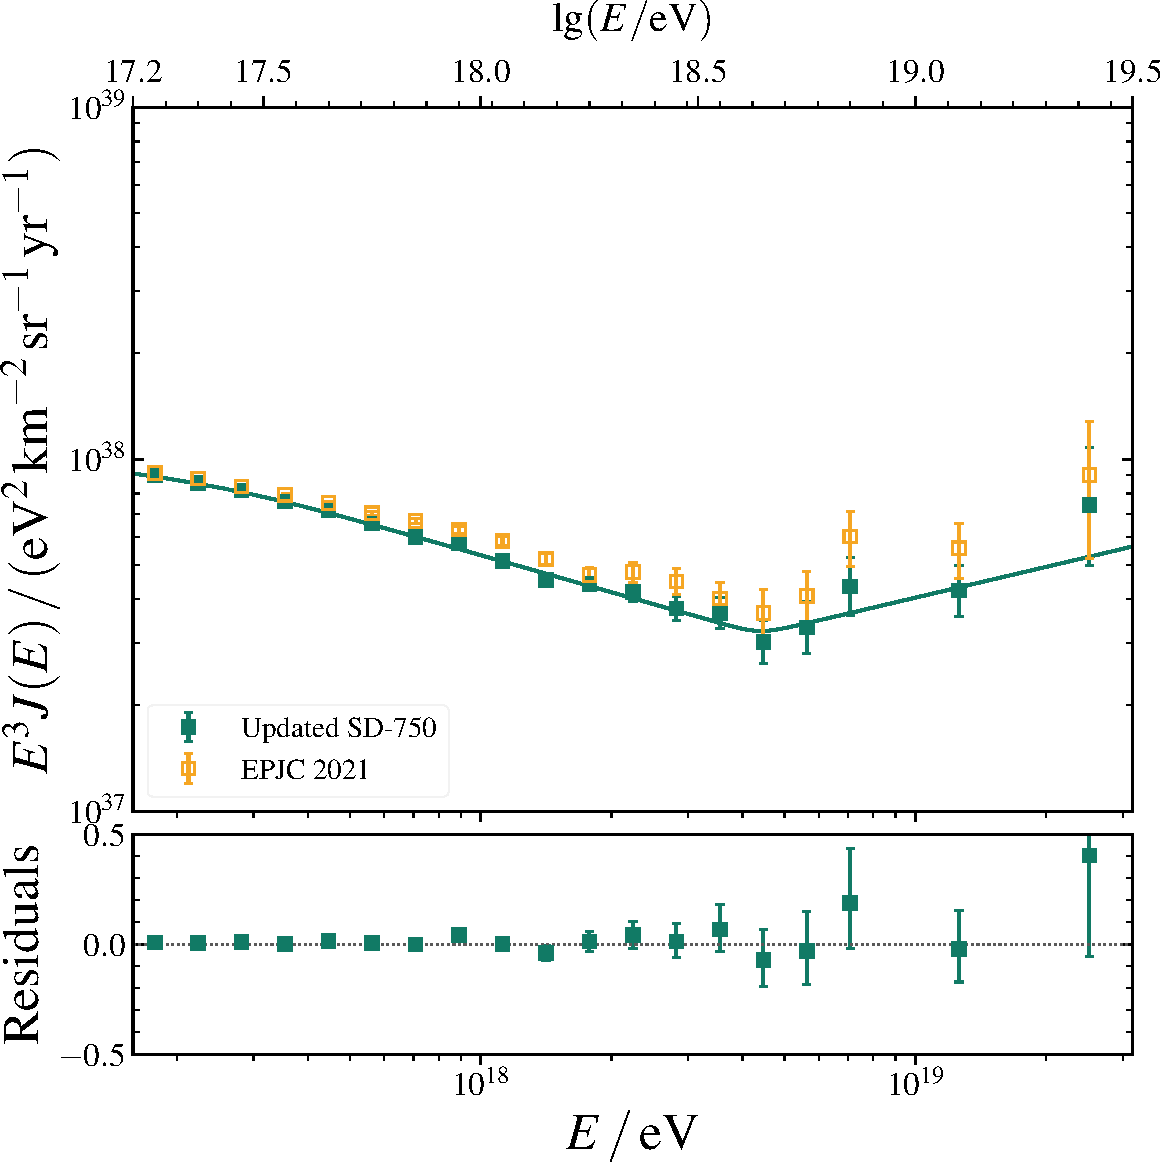
\includegraphics[width=0.90\linewidth]{figures/chapter_combined/sd750_unfolded_spectrum.pdf}
    \caption{Unfolded cosmic-ray spectrum measured with the updated \sd{750} dataset and its best-fit spectral model, obtained for $\lg(E/\mathrm{eV})\geq17.2$ with the second-knee position fixed to the \sd{433} result. The open squares show the unfolded spectrum reported in \cite{PierreAuger:2021:InfillSpectrum} for comparison. The lower panel shows the residuals of the updated \sd{750} points with respect to the fitted model; the published points are not included in the residuals. Only statistical uncertainties are shown.}
    \label{fig:sd750_unfolded_spectrum}
\end{figure}

\begin{table}
    \centering
    \caption{Parameters of the standalone \sd{750} spectrum fit for $\lg(E/\mathrm{eV})\geq17.2$. The second-knee position is fixed to the \sd{433} result and the ankle width is fixed to $\omega_{12}=0.05$. The quoted uncertainties are statistical.}
    \label{tab:sd750_fit_parameters}
    \begin{tabular}{lc}
        \toprule
        Parameter & Value\\
        \midrule
        $J_0\,/\,(10^{-13}\,\mathrm{km}^{-2}\,\mathrm{sr}^{-1}\,\mathrm{yr}^{-1}\,\mathrm{eV}^{-1})$ & $0.986\pm0.008$\\
        $\lg(E_{01}/\mathrm{eV})$ & $17.44$ (fixed)\\
        $\omega_{01}$ & $0.26\pm0.16$\\
        $\gamma_0$ & $3.16\pm0.03$\\
        $\gamma_1$ & $3.35\pm0.02$\\
        $\lg(E_{12}/\mathrm{eV})$ & $18.64\pm0.09$\\
        $\omega_{12}$ & $0.05$ (fixed)\\
        $\gamma_2$ & $2.71\pm0.18$\\
        \bottomrule
    \end{tabular}
\end{table}

\section{The Combined Spectrum}
\label{sec:combined_spectrum}

To combine the larger exposure of the \sd{750} with the lower energy threshold of the \sd{433}, the procedure used in Refs.~\cite{PierreAuger:2021:InfillSpectrum,PierreAuger:2025:Declination} is followed. The \sd{433} and \sd{750} spectra are reconstructed separately and enter the combination with their respective event distributions, exposures, and detector-response matrices. The exposure of each array is calculated from its geometrical aperture above the corresponding full-efficiency threshold, as described in \cref{sec:exposure}.
The combined likelihood is defined as
\begin{align}
    \mathcal{L}
    \left(
    \mathbf{s},
    \delta\mathcal E_{433},
    \delta A,
    \delta B
    \right)
    =
    \mathcal{L}_{\mathrm{SD\text{-}433}}\,
    \mathcal{L}_{\mathrm{SD\text{-}750}}\,
    \mathcal{L}_{\mathrm{exp}}\,
    \mathcal{L}_{AB},
\end{align}
\noindent where $\mathbf{s}$ denotes the spectral parameters and $\mathcal{L}_{\mathrm{SD\text{-}433}}$ and $\mathcal{L}_{\mathrm{SD\text{-}750}}$ are the likelihoods of the two arrays defined in \cref{sec:unfolded_spectrum}.
The exposure term allows the fitted \sd{433} exposure to vary around its nominal value:
% \begin{align}
%     \mathcal{L}(\delta\mathcal{E}_{\text{SD-433}})=\frac{1}{\sigma_{\mathcal{E}_{\text{SD-433}}}\sqrt{2\pi}}\exp\left(
%     -\frac{\mathcal{E}_{\text{SD-433}}-\delta\mathcal{E}}{\sigma_{\mathcal{E}_{\text{SD-433}}}}
%     \right)^2
% \end{align}

\begin{align}
\mathcal L_{\mathrm{exp}}(\delta\mathcal E_{433})
&=
\frac{1}{\sqrt{2\pi}\,\sigma_{\mathcal E}}
\exp\left[
-\frac{1}{2}
\left(
\frac{\delta\mathcal E_{433}}{\sigma_{\mathcal E}}
\right)^2
\right],
\end{align}
\noindent where
\begin{align}
\delta\mathcal E_{433}
&\equiv
\widehat{\mathcal E}_{433}-\mathcal E_{433}
\end{align}
\noindent and $\sigma_{\mathcal E}=0.03\,\mathcal E_{433}$ is the $3\%$ uncertainty assigned to the nominal exposure~\cite{PierreAuger:2010:TriggerAperture}.
The Gaussian term penalizes deviations of the fitted exposure from its nominal value.
Because the \sd{433} energy scale is calibrated against the \sd{750}, the relative calibration is allowed to vary through shifts in $A$ and $B$.
These shifts are defined as
\begin{align}
\delta A&\equiv\widehat A-A,
&
\delta B&\equiv\widehat B-B,
\end{align}
\noindent where $A$ and $B$ are the nominal calibration parameters and $\widehat A$ and $\widehat B$ their fitted values.
Their systematic uncertainties and correlation are incorporated through the bivariate Gaussian constraint
\begin{align}
\mathcal L_{AB}(\delta A,\delta B)
&=
\frac{1}{2\pi\sigma_A\sigma_B\sqrt{1-\rho_{AB}^{2}}}
\exp\left[
-\frac{1}{2(1-\rho_{AB}^{2})}
\left(
\frac{\delta A^{2}}{\sigma_A^{2}}
+\frac{\delta B^{2}}{\sigma_B^{2}}
-\frac{2\rho_{AB}\delta A\,\delta B}{\sigma_A\sigma_B}
\right)
\right],
\end{align}
\noindent where $\sigma_A$, $\sigma_B$, and $\rho_{AB}$ are obtained from the calibration analysis in \cref{sec:calibration}.
This term constrains the calibration shifts according to their uncertainties while preserving their correlation.

Variations in the \sd{433} exposure and in the calibration normalization $A$ both affect the relative flux normalization and therefore cannot be constrained simultaneously.
The combination is consequently performed in two steps.
First, the spectral parameters and $\delta\mathcal E_{433}$ are fitted while $A$ and $B$ remain fixed.
The exposure is then fixed to its best-fit value, and the fit is repeated with $\delta A$ and $\delta B$ as free parameters.
The results of both fits are summarized in \cref{table:combined_parameters_single}.

\begin{table}
    \centering
    \caption{Combined \sd{433}-\sd{750} fit results. The shifts $\delta\mathcal E_{433}$, $\delta A$, and $\delta B$ are relative to $\mathcal E_{433}=2.88\,\mathrm{km^2\,sr\,yr}$, $A=149.49\,\mathrm{PeV}$, and $B=0.963$. In the exposure-only fit, only the exposure shift varies; in the calibration-variation fit, the exposure shift is fixed to the preceding best-fit value and the calibration shifts vary. The ankle width is fixed to $\omega_{12}=0.05$ in both fits. The uncertainties on $\delta A$ and $\delta B$ are obtained from a likelihood profile in these parameters.}
    \label{table:combined_parameters_single}
    \begin{tabular}{lcc}
        \toprule
        Parameter & Exposure only & Calibration variation\\
        \midrule
        $J_0\,/\,(10^{-13}\,\mathrm{km}^{-2}\,\mathrm{sr}^{-1}\,\mathrm{yr}^{-1}\,\mathrm{eV}^{-1})$ & $0.952\pm0.039$ & $0.992\pm0.017$\\
        $\lg(E_{01}/\mathrm{eV})$ & $17.23\pm0.09$ & $17.17\pm0.02$\\
        $\omega_{01}$ & $0.31\pm0.11$ & $0.39\pm0.04$\\
        $\gamma_0$ & $2.94\pm0.07$ & $2.87\pm0.03$\\
        $\gamma_1$ & $3.34\pm0.02$ & $3.35\pm0.01$\\
        $\lg(E_{12}/\mathrm{eV})$ & $18.61\pm0.11$ & $18.60\pm0.11$\\
        $\omega_{12}$ & $0.05$ (fixed) & $0.05$ (fixed)\\
        $\gamma_2$ & $2.88\pm0.18$ & $2.88\pm0.19$\\
        \midrule
        $\delta\mathcal E_{433}\,/\,(\mathrm{km^2\,sr\,yr})$ & $-0.04\pm0.03$ & $-0.04$ (fixed)\\
        $\delta A/\mathrm{PeV}$ & $0$ (fixed) & $0.1\pm6.1$\\
        $\delta B$ & $0$ (fixed) & $-0.003\pm0.027$\\
        \midrule
        $D^2/\mathrm{dof}$ & $36.31/30$ & $29.98/29$\\
        $p$-value & $0.198$ & $0.415$\\
        \bottomrule
    \end{tabular}
\end{table}
The combined spectrum is shown with purple triangles in \cref{fig:sd433_sd750_combined_spectrum}, together with the \sd{433} spectrum in red circles and the \sd{750} spectrum in green squares.
The \sd{433} data constrain $\gamma_0$ at the lowest energies, while both measurements contribute to determining the second-knee energy, the transition width $\omega_{01}$, and the spectral index $\gamma_1$.
The fitted value of $\gamma_1$ is compatible with the standalone measurements from both arrays.
At higher energies, the larger exposure of the \sd{750} constrains the ankle position, although $\gamma_2$ remains loosely constrained.
In the calibration-variation fit, the resulting shifts are $\delta A=0.1\pm6.1\,\mathrm{PeV}$ and $\delta B=-0.003\pm0.027$, with uncertainties obtained from a likelihood profile in the $(\delta A,\delta B)$ parameter space.
Both shifts are compatible with zero, showing that the combination does not require a significant relative recalibration of the \sd{433} and \sd{750} energy scales.
The spectral parameters remain compatible with those obtained in the exposure-only fit.
Therefore, the combined result is stable under the allowed calibration variations, while the relative normalization is primarily accommodated by the fitted \sd{433} exposure shift.

The likelihood fit is performed using the event distributions of the two arrays separately.
For presentation, the combined flux is constructed after the fit by adding their unfolded event counts,
\begin{align}
    J_i^{\mathrm{comb}}=
    \frac{n_i^{433}c_i^{433}+n_i^{750}c_i^{750}}
    {\Delta E_i\,\mathcal E_{\mathrm{eff},i}},
\end{align}
\noindent where $n_i^x$ is the number of events measured by array $x$ in bin $i$, and $c_i^x$ is the corresponding correction factor calculated from the fitted spectrum and detector-response matrix.
Terms from an array outside its selected energy range are omitted.
The effective exposure is
\begin{align}
\mathcal E_{\mathrm{eff},i}=
\begin{cases}
\mathcal E_{433}+\delta\mathcal E_{433},
& \text{only the \sd{433} contributes},\\
\mathcal E_{750}+\mathcal E_{433}+\delta\mathcal E_{433},
& \text{both arrays contribute},\\
\mathcal E_{750},
& \text{only the \sd{750} contributes}.
\end{cases}
\end{align}

\begin{figure}
    \centering
    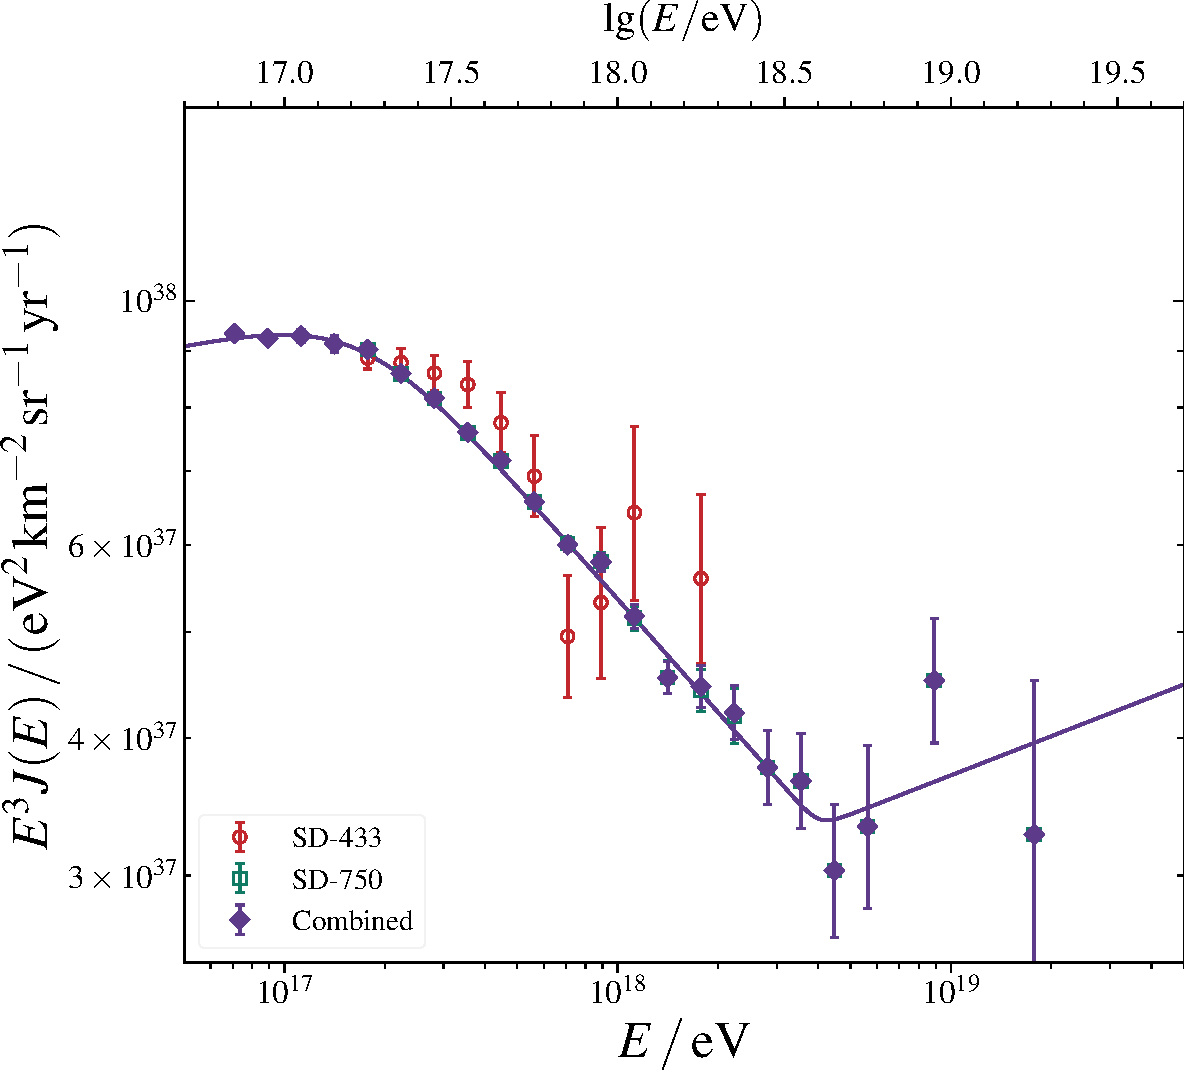
\includegraphics[width=0.82\linewidth]{figures/chapter_combined/sd433_sd750_combined_spectrum.pdf}
    \caption{Unfolded spectra measured with the \sd{433} and \sd{750}, together with the combined spectrum and common best-fit model. The combined spectrum uses the \sd{433} binning below $\lg(E/\mathrm{eV})=17.2$ and the \sd{750} binning at higher energies. Only statistical uncertainties are shown.}
    \label{fig:sd433_sd750_combined_spectrum}
\end{figure}

To assess the stability of the combined result, the lower boundary of the \sd{750} fit range was varied from $\lg(E_{\min}^{750}/\mathrm{eV})=17.0$ to $17.5$, while the upper boundary was kept fixed at $19.4$.
The results are shown in \cref{fig:combined_fit_min_scan}.
The fit ranges starting at $17.0$ and $17.1$ extend below the full-efficiency threshold of the \sd{750} and yield $p$-values below $0.05$.
The fit first becomes acceptable at $17.2$, which coincides with the full-efficiency threshold.
Although the $p$-value reaches its maximum at $17.3$, the fitted second-knee energies are compatible across the accepted thresholds.
We therefore retain $17.2$ as the nominal lower boundary, maximizing the \sd{750} event sample while restricting the fit to the full-efficiency range.

\begin{figure}
    \centering
    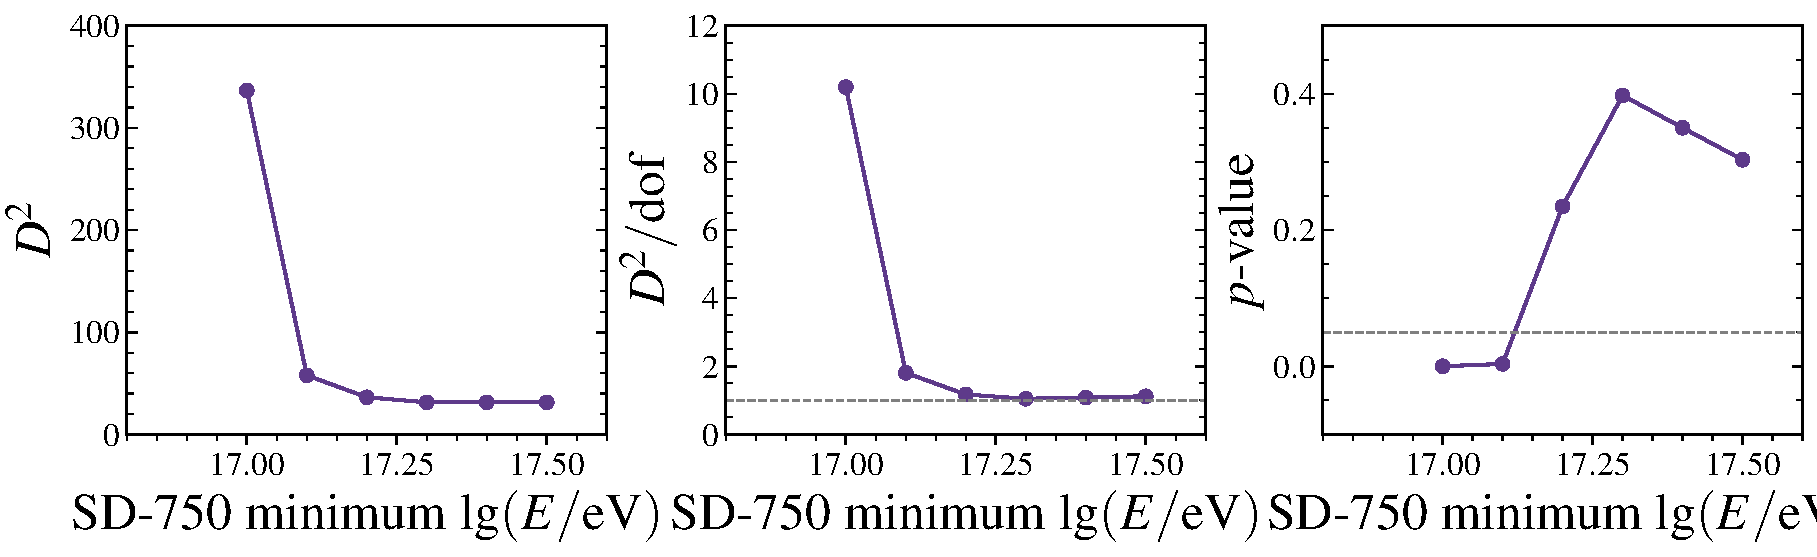
\includegraphics[width=\linewidth]{figures/chapter_combined/combined_fit_min_scan_deviance.pdf}
    \caption{Dependence of the combined-fit $p$-value, second-knee energy, and spectral indices $\gamma_0$ and $\gamma_1$ on the minimum \sd{750} energy included in the fit. The dashed line in the upper-left panel indicates $p=0.05$. The \sd{750} upper boundary is fixed at $\lg(E/\mathrm{eV})=19.4$, the \sd{433} fit range is unchanged, and the \sd{433} exposure is fixed to the value preferred by the nominal combined fit.}
    \label{fig:combined_fit_min_scan}
\end{figure}

The upper boundary of the \sd{750} fit range was then varied while the lower boundary was kept fixed at $\lg(E_{\min}^{750}/\mathrm{eV})=17.2$.
The results are shown in \cref{fig:combined_fit_max_scan}.
All tested ranges give acceptable $p$-values, with the maximum occurring at $\lg(E_{\max}^{750}/\mathrm{eV})=19.0$.
As higher-energy events are included, the ankle position and $\gamma_2$ become more stable and their uncertainties decrease.
We therefore choose $19.4$ as the nominal upper boundary to include the available high-energy events and better constrain the spectrum above the ankle.
The spectral parameters obtained with this fit range are compatible with the previous Auger measurement in Ref.~\cite{PierreAuger:2021:InfillSpectrum}.

\begin{figure}
    \centering
    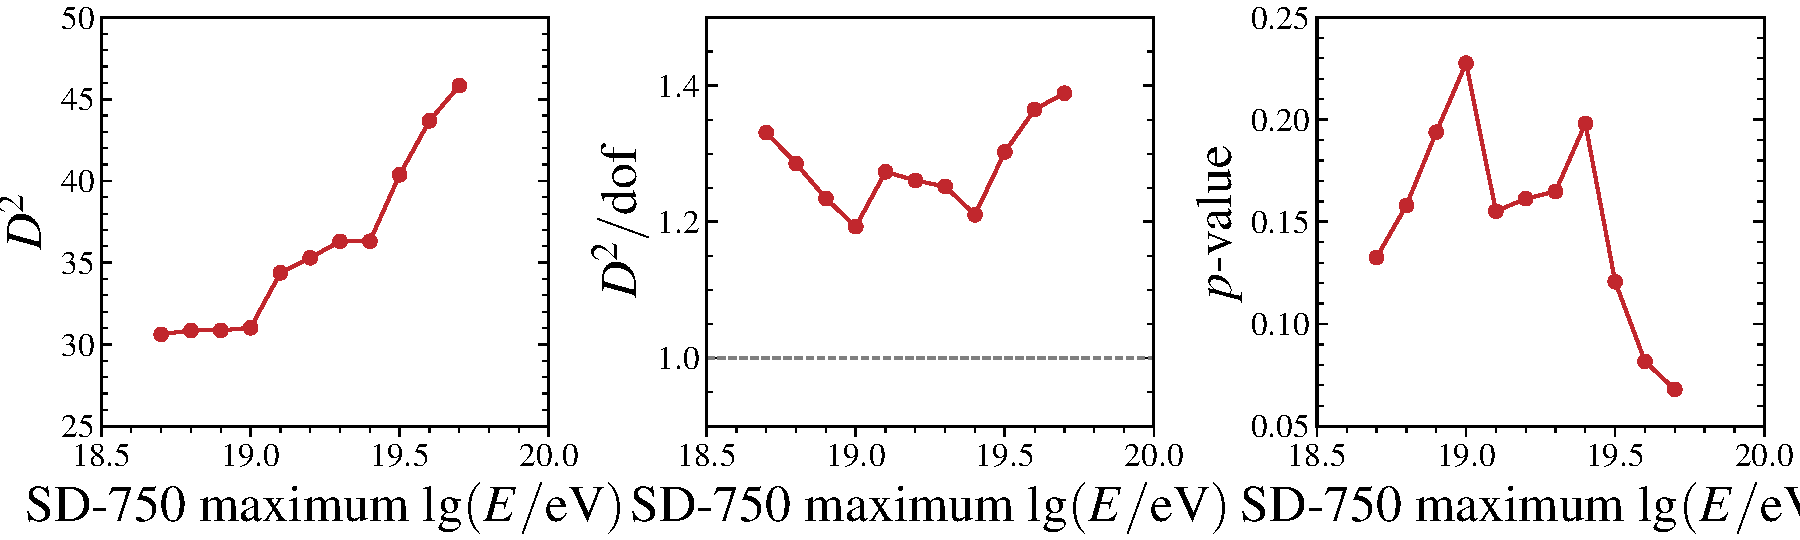
\includegraphics[width=\linewidth]{figures/chapter_combined/combined_fit_max_scan_deviance.pdf}
    \caption{Dependence of the combined-fit $p$-value, ankle energy, and spectral indices $\gamma_1$ and $\gamma_2$ on the maximum \sd{750} energy included in the fit. The dashed line in the upper-left panel indicates $p=0.05$. The \sd{750} lower boundary is fixed at $\lg(E/\mathrm{eV})=17.2$.}
    \label{fig:combined_fit_max_scan}
\end{figure}

With the fit ranges fixed to $16.8\leq\lg(E^{433}/\mathrm{eV})\leq18.2$ and $17.2\leq\lg(E^{750}/\mathrm{eV})\leq19.4$, the systematic uncertainties of the combined spectrum are evaluated using the methods described in \cref{sec:systematics}.
The dominant contribution to the flux uncertainty comes from the \gls{fd} energy scale, which is common to both arrays.
Its effect is propagated using \cref{eq:energy_systematic_bplwst} and is shown by the shaded band in \cref{fig:sd433_sd750_combined_systematic}.
The same energy-scale uncertainty is propagated to the second-knee and ankle energies, $E_{01}$ and $E_{12}$.
The systematic uncertainties of the spectral indices $\gamma_0$, $\gamma_1$, and $\gamma_2$ are inherited from the uncertainty in the calibration slope and are evaluated using the analytical expression in \cref{eq:calibration_spectral_index_change}.
Finally, the systematic uncertainty assigned to $\omega_{01}$ is the maximum variation observed in the \sd{750} minimum-energy scan.
The resulting spectral parameters and their statistical and systematic uncertainties are summarized in \cref{table:combined_spectrum_parameters_systematics}.





\begin{figure}
    \centering
    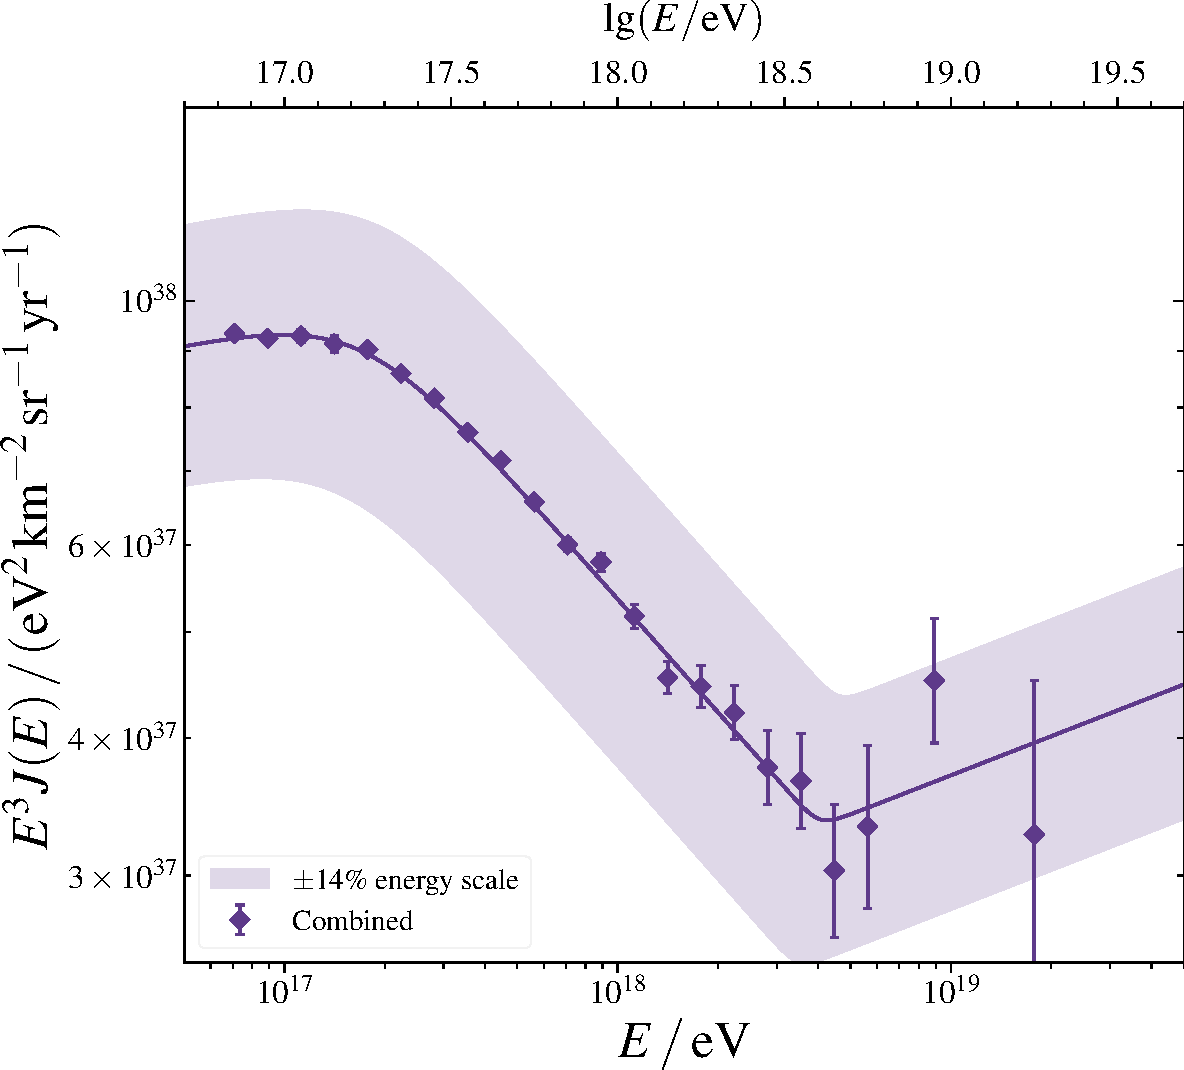
\includegraphics[width=0.8\linewidth]{figures/chapter_combined/sd433_sd750_combined_spectrum_systematic.pdf}
    \caption{Combined \sd{433}--\sd{750} spectrum and common best-fit model. The shaded region shows the effect of the $\pm14\%$ energy-scale uncertainty propagated through the fitted spectrum using \cref{eq:energy_systematic_bplwst}. The error bars represent statistical uncertainties.}
    \label{fig:sd433_sd750_combined_systematic}
\end{figure}

\begin{table}
    \centering
    \caption{
        Best-fit values of the combined \sd{433}--\sd{750} spectral parameters
        from the exposure-only fit. The first uncertainty is statistical and
        the second systematic.
    }
    \label{table:combined_spectrum_parameters_systematics}
    \begin{tabular}{lc}
        \hline
        Parameter & Value $\pm\sigma_{\mathrm{stat}}\pm\sigma_{\mathrm{syst}}$ \\
        \hline
        $J_0/\left(\mathrm{km^{-2}\,yr^{-1}\,sr^{-1}\,eV^{-1}}\right)$
        & $(0.952\pm0.039\pm0.284)\times10^{-13}$ \\
        $\gamma_0$ & $2.94\pm0.07\pm0.12$ \\
        $E_{01}/\mathrm{PeV}$ & $170\pm35\pm24$ \\
        $\gamma_1$ & $3.34\pm0.02\pm0.14$ \\
        $\omega_{01}$ & $0.31\pm0.11\pm0.09$ \\
        $E_{12}/\mathrm{EeV}$ & $4.0\pm1.2\pm0.6$ \\
        $\gamma_2$ & $2.88\pm0.18\pm0.11$ \\
        $\omega_{12}$ & $0.05$ -- fixed \\
        \hline
    \end{tabular}
\end{table}

\section{Summary}

This chapter presents an updated \sd{750} dataset and spectrum measurement.
The detection efficiency is determined with a data-driven method using events recorded by both the \sd{433} and \sd{750}, yielding a full-efficiency threshold of $\lg(E/\mathrm{eV})=17.2$.
The detector response is modeled using the same method as for the \sd{433} and is used to unfold the measured spectrum.
Because the \sd{750} fit range begins close to the second knee, its position is fixed to the single \sd{433} result in the fit.
In a cross-check where the second-knee position is allowed to vary, the fitted value remains compatible with the \sd{433} measurement.
The larger collecting area of the \sd{750} extends the spectrum measurement through the ankle and allows the second-knee transition width to be fitted, although $\gamma_2$ remains loosely constrained.
The updated \sd{750} spectrum is then combined with the \sd{433} measurement.
The likelihood retains the separate event distributions of the two arrays and includes nuisance terms for the \sd{433} exposure and relative energy calibration.
The profiled shifts in the calibration parameters $A$ and $B$ are compatible with zero, indicating that no significant relative recalibration is required.
The exposure-only fit gives $\delta\mathcal E_{433}=-0.04\pm0.03\,\mathrm{km^2\,sr\,yr}$, which is compatible with zero within approximately $1.5\sigma$.
For presentation, the combined flux is constructed from the sum of the unfolded event counts and the corresponding effective exposure.
The combined fit favors a lower second-knee energy than the standalone \sd{433} measurement, with $\lg(E_{01}/\mathrm{eV})=17.23\pm0.09$.
This result is sensitive to the minimum \sd{750} energy included in the fit.
The nominal boundary, $\lg(E_{\min}^{750}/\mathrm{eV})=17.2$, is retained because it corresponds to the measured full-efficiency threshold and is the lowest boundary for which the combined fit is acceptable.
The statistical interval on $\lg(E_{01}/\mathrm{eV})$ spans approximately one energy bin.
The combined fit also favors a broader transition, $\omega_{01}=0.31\pm0.11$, than the standalone best-fit value, $\omega_{01}=0.09\pm0.27$, although the two measurements are statistically compatible.
The unfolded \sd{433} and \sd{750} spectra show a possible difference in flux normalization in their overlap region, but its statistical significance is insufficient to establish a discrepancy.
The combined fit therefore characterizes both the second knee and the ankle, providing a \gls{sd} spectrum measurement that spans almost three decades in energy.
% \section{Combined SD-433 and SD-750 spectrum}
% \label{sec:combined_spectrum}

% \begin{figure}
%     \centering
%     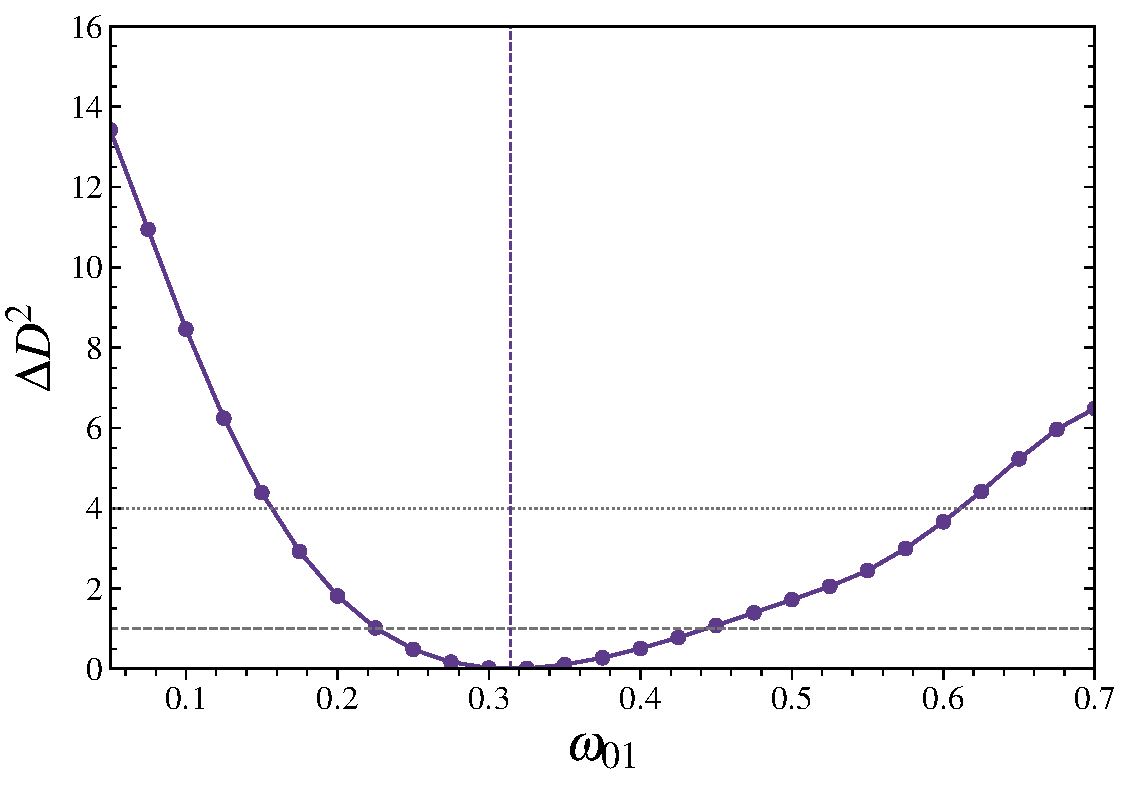
\includegraphics[width=0.8\linewidth]{figures/chapter_combined/combined_omega_profile.pdf}
%     \caption{Profile of the combined-fit Poisson deviance as a function of the second-knee transition width $\omega_{01}$. At each fixed value of $\omega_{01}$, the remaining spectral parameters are profiled, while the \sd{433} exposure is fixed to the value preferred by the nominal combined fit and the calibration parameters are left unchanged. The horizontal lines indicate $\Delta D^2=1$ and $4$, and the vertical dashed line marks the best-fit value $\omega_{01}=0.314$.}
%     \label{fig:combined_omega_profile}
% \end{figure}

\end{document}
